\begin{wrapfigure}{r}{8cm}
  \centering
  \vspace{-30px}
  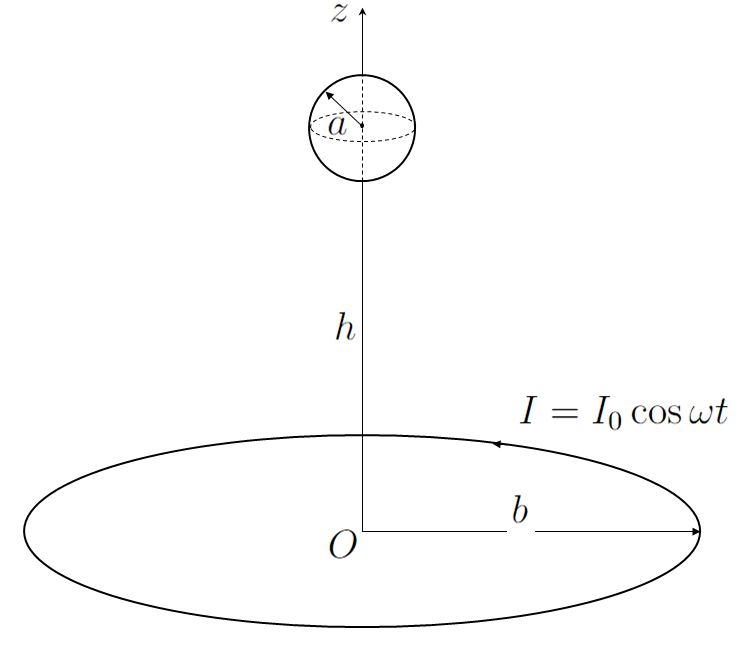
\includegraphics[width=0.45\textwidth]{images/Hinh 6.PNG}
  \vspace{-20px}
  \begin{center}
    \figurename{ 6}
  \end{center}
\end{wrapfigure}

\vspace{-30px}
\noindent Khi một vật dẫn điện được đặt trong từ trường biến thiên, dòng điện Foucault (dòng điện xoáy) sẽ xuất hiện bên trong nó. Dòng Foucault có thể tạo ra tác dụng nhiệt được sử dụng để nung nóng và rèn kim loại; bên cạnh đó, tác dụng cơ của dòng điện này còn được ứng dụng để hãm chuyển động, truyền động, treo các vật thể dẫn điện,\dots. Để nghiên cứu hai tác dụng nêu trên của dòng điện xoáy, ta sẽ sử dụng một thiết bị như hình 6: một cuộn dây bán kính $b$ được đặt cố định trên mặt bàn nằm ngang, mang dòng điện xoay chiều có cường độ $I(t)=I_{0}\cos\omega t$. Một quả cầu dẫn điện có trọng lượng $G$, bán kính $b$, độ dẫn điện $\sigma$ được đặt sao cho tâm quả cầu nằm trên trục đối xứng của vòng dây, cách tâm vòng dây một khoảng $h\ll a$. Giả sử $a\ll b$ và độ sâu bề mặt của quả cầu là $\sigma=\sqrt{\dfrac{2}{\omega\mu_{9}\sigma}}\ll a$ với $\mu_{0}$ là độ từ thẩm trong chân không. Bỏ qua hiện tượng bức xạ điện từ.
\begin{enumerate}
  \item Đặt một quả cầu dẫn lý tưởng $(\sigma)\rightarrow\infty$ bán kính $a$ trong một từ trường đều và ổn định $\vec{B}_{e}=B_{e}\hat{z}$, dòng điện từ hoá bên trong quả cầu sẽ tạo ra một từ trường $\vec{B}'$ bên ngoài quả cầu, từ trường này tương tự với từ trường do một lưỡng cực từ lý tưởng đặt tại tâm quả cầu tạo ra:
        \begin{equation*}
          \vec{B}'=\frac{\mu_{0}}{4\pi}\frac{3(\vec{m}\cdot\hat{r})\hat{r}-\vec{m}}{r^{3}}
        \end{equation*}
        trong đó $\vec{m}$ là momen lưỡng cực từ của lưỡng cực, cũng là momen lưỡng cực của quả cầu dẫn lý tưởng này. Xem $\vec{B}_{e}$ như một đại lượng đã biết, xác định $\vec{m}$ và phân bố dòng điện trên bề mặt quả cầu dẫn.
  \item Xác định cảm ứng từ $\vec{B}$ do dòng điện trong dây dẫn tạo ra tại tâm quả cầu vào thời điểm $t$.
  \item Xác định giá trị của $I_{0}$ để quả cầu có thể cân bằng tại vị trí như hình 6. Giả sử $I_{0}$ đủ lớn để biên độ dao động của quả cầu dẫn quanh vị trí cân bằng có thể bỏ quả. Cho biết: Nếu momen từ $\vec{m}$ của lưỡng cực từ và từ trường ngoài $\vec{B}_{e}$ tại vị trí của lưỡng cực có phương song song với $Oz$, các thành phần tương ứng của chúng là $m$ và $B_{e}=B_{e}(z)$ thì lực tác dụng lên lưỡng cực có dạng:
        \begin{equation*}
          \vec{F}=m\frac{dB_{e}}{dz}\hat{z}
        \end{equation*}
  \item Khi khảo sát tác dụng nhiệt của dòng điện xoáy, ta phải xét đến hiệu ứng bề mặt của quả cầu dẫn. Giả sử dòng điện xoáy được phân bố đều trên phương bán kính trong độ sâu bề mặt và bằng không ở mọi nơi khác bên trong quả cầu. Xác định biểu thức gần đúng của nhiệt năng trung bình do quả cầu toả ra trong một chu kỳ.
\end{enumerate}